\section{Current}
Current ($i$) is the force that moves charge through a circuit. Current can be defined as an amount of charge moved over a time interval. This can be expressed as the following relation:
\begin{align}
i(t)=\dfrac{dq(t)}{dt} \Leftrightarrow q(t)=\int i(t)\ dt,
\label{I=dq/dt}
\end{align}
%REFERENCE MED SIDETAL!!!!
where $i(t)$ is the current (in ampere, $A$) to a given time (in seconds, $s$), and $q(t)$ is the function for charge at a given time $t$ (in coulomb, C). 
\\
There are two types of current: alternating current (AC) and direct current (DC). Per definition, DC current is a constant flow of current, while AC alternates (see figure \ref{fig:ACDC}). 
\begin{figure}[H] 
\begin{tikzpicture}
\begin{axis}[ticks=none,
axis lines =center,
xlabel={t},
ylabel={i(t)},
    height=7cm, width=9cm,
    xmin=0, xmax=10, ymin=-2, ymax=2]
\addplot [
    domain=0:10, 
    samples=100, 
    color=red,
]
{1};
\addlegendentry{$DC$}
\addplot [
    domain=0:10, 
    samples=100, 
    color=blue,
    ]
    {sin(\x r)};
\addlegendentry{$AC$}
\end{axis}
\end{tikzpicture}
\caption{AC and DC current versus time.}
\label{fig:ACDC}
\end{figure}
\noindent
A sinusoidal AC current can be described with the function: 
\begin{align}
i\left(t, f, A, \theta\right) =& A\cdot \sin{\left(2\pi ft + \theta\right)}, \nonumber
\\
=& A \cdot \sin{\left(\omega t + \theta\right)}, \label{eq:omega}
\end{align}
where $f$ is frequency (in Hertz, $Hz$), $t$ is time (in seconds, $s$), $Hz$), which is cycles per second, $\omega = 2\pi f$ (in rads per second), $A$ is amplitude (a scalar, that has the same unit as the function), and $\theta$ is the phase shift (in seconds, $s$).
For ease of understanding, $\omega$ is sometimes used for notation instead of $2\pi f$. $\omega$ is also called the angular frequency of the signal.
Equation \ref{eq:omega} can be plotted as such:
\begin{figure}[H]
	\centering
	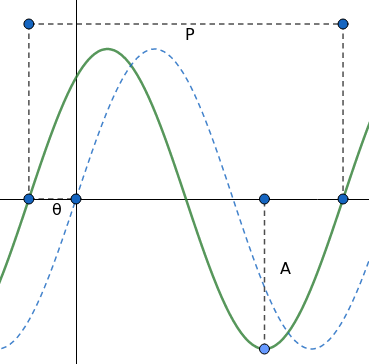
\includegraphics[scale=0.7]{fig/img/AC.png}
	\caption{An AC current, shown in green. The current has been phase shifted by $\theta$. The current has amplitude $A$, and period $P=f^{-1}$. The dotted blue line \ref{eq:omega} shows the same current with $\text{phase shift} =0$.}
\end{figure}


\section{Voltage}
Voltage ($v$), also called electric potential difference, is the change in potential energy that a charge undergoes, when it passes through two given points in a circuit. This is expressed in the following equation:
\begin{align*}
	v=\dfrac{dU(q)}{dq},
\end{align*}
\\
where $U(q)$ is the function for potential energy (in joules, $J$) with given a charge $q$.



\section{Resistor}
When a resistor ($R$), which is a passive element, is added to the circuit, it creates a resistance. Resistance makes it more difficult for the current to pass through the element. Resistance is defined as the proportional constant between current and voltage. The mathematical relation of this is given by:
\begin{align} 
\label{Ohm}
v(t)=R\cdot i(t),\ R\geq0,
\end{align}
where $R$ is resistance (in Ohm, $\Omega$). Furthermore, the power (in watts, $w$) can be expressed as: \cite[p. 25]{bcircuit} 
\begin{align} 
\label{power}
p(t)=v(t)\cdot i(t).
\end{align}
By inserting this in \eqref{Ohm}, the following expression is found:
\begin{align}
p(t)&=Ri(t)\cdot i(t), \nonumber \\
p(t)&=R \cdot i^2(t), \nonumber \\
p(t)&=R \cdot \left(\dfrac{v(t)}{R} \right)^2, \nonumber \\
p(t)&=\dfrac{v^2(t)}{R}. \label{resistor:power}
\end{align}
This is defined as the amount of work done per second.


\section{Capacitor}
A capacitor ($C$), which is a passive element, consists of two similar sized plates. When a voltage is applied to the circuit, the capacitor gets charged. The capacitance is the amount of energy a capacitor can store, when it is fully charged. The capacitor gets charged, when a positive charge is transferred from one plate to another through the circuit.
\\
The capacitance is given by the following equation:
\begin{align*}
C=\dfrac{\epsilon_{0}A}{d},
\end{align*}
where $C$ is the capacitance (in farad, $F$) and $\epsilon_{0}$ is the permittivity of free space, which is equal to $8.85 \cdot 10^{-12}                                                 \frac{F}{m}$. $A$ is the surface area of the plates (in square meters, $m^{2}$), and $d$ is the distance between the two plates (in meters, $m$).
\\
The charge of a capacitor across a voltage ($v$) and capacitance ($C$) is equal to:
\begin{align}
\label{QCV}
q_C(t) = Cv_C(t).	
\end{align}
From \eqref{I=dq/dt}, current is defined as:
\begin{align*}
	i(t) = \frac{dq(t)}{dt}.
\end{align*}
Equation \eqref{QCV} is used:
\begin{align*}
	i_C(t) = \frac{d}{dt}\big(Cv_C(t)\big).
\end{align*}
For a capacitor with a capacitance $C$, the current can be written as:
\begin{align}
	i_C(t) = C\frac{dv_C(t)}{dt}.\label{iC}
\end{align}


\section{Time constant ($\tau$)}
%A constant that shows up when looking at RC circuits, is the time constant $\tau = R \cdot C$, where $R$ is the resistance of the resistor, $C$ is the capacitance of the capacitor, and $\tau$ is time (in seconds, $s$).

The product of the resistance and capacitance is a useful  constant when looking at RC circuits. This constant is written as: $\tau = R \cdot C$, and is measured in time (in seconds, $s$)